\section{GTFS}
\label{sec:gtfs}

The adoption of GTFS \citep{GoogleDevelopers_2006} by public transport agencies around the world has made it possible for applications such as Google Maps to access and display public transport data to users, regardless of their location. The main goal of GTFS is to specify, in detail, how transit data should be organised so that it is consistent across agencies around the world. As a result, it does not matter whether you are in Auckland, Paris, or C\'ordoba; Google Maps can show you public transport directions by accessing local \gls{gtfs} data.


\GTFS{} consists of two components, \emph{static} and \emph{real-time}.\footnote{The official name is `GTFS-realtime'.} The static component specifies how information about the schedule, fares, and route geography are organised, while the \emph{real-time} component specifies the format for real-time data: vehicle locations, stop updates and \glspl{eta}, and service advisories. Each of the static and real-time components is implemented by the transit provider; for example \AT{}'s \GTFS{} service is hosted at \url{https://dev-portal.at.govt.nz}.


\subsection{Static GTFS}
\label{sec:gtfs_static}


\begin{table}[t]
\centering
\fontsize{10}{12}\selectfont
\begin{tabular}{ll}
\toprule
Term & Definition \\
\midrule
route & a collection of \emph{trips} that are displayed to comuters
as a single service \\
trip & a journey servicing two or more stops at a specific time \\
stop & a location where passengers are picked up or dropped off \\
stop time & the (scheduled) times at which vehicles
will arrive at stops for each trip \\
shape & the GPS track a vehicle will take for a specific route \\
\bottomrule
\end{tabular}
\caption[Definitions of GTFS terms]{Definitions of the relevant GTFS terms from \url{https://developers.google.com/transit/gtfs/reference/}}
\label{tab:gtfs_terms}
\end{table}


There are several components of GTFS that are of particular interest to us: routes, trips, stops, stop times, and shapes. The definitions of these terms are given in \cref{tab:gtfs_terms}. Extensive documentation can be found on the GTFS website.\footnote{\url{https://developers.google.com/transit/gtfs/}}


\Cref{fig:gtfs_nw} demonstrates a single \emph{route} along which there are two active \emph{trips} (A and B). The route's \emph{shape} is represented by the line connecting the six \emph{stops} numbered 1--6. The real-time arrivals board or \gls{dms} is shown for stop~5, displaying the scheduled \emph{stop time} (arrival time) for each trip at that stop. The additional information displayed is described in the next section.



\begin{knitrout}\small
\definecolor{shadecolor}{rgb}{0.969, 0.969, 0.969}\color{fgcolor}\begin{figure}

{\centering 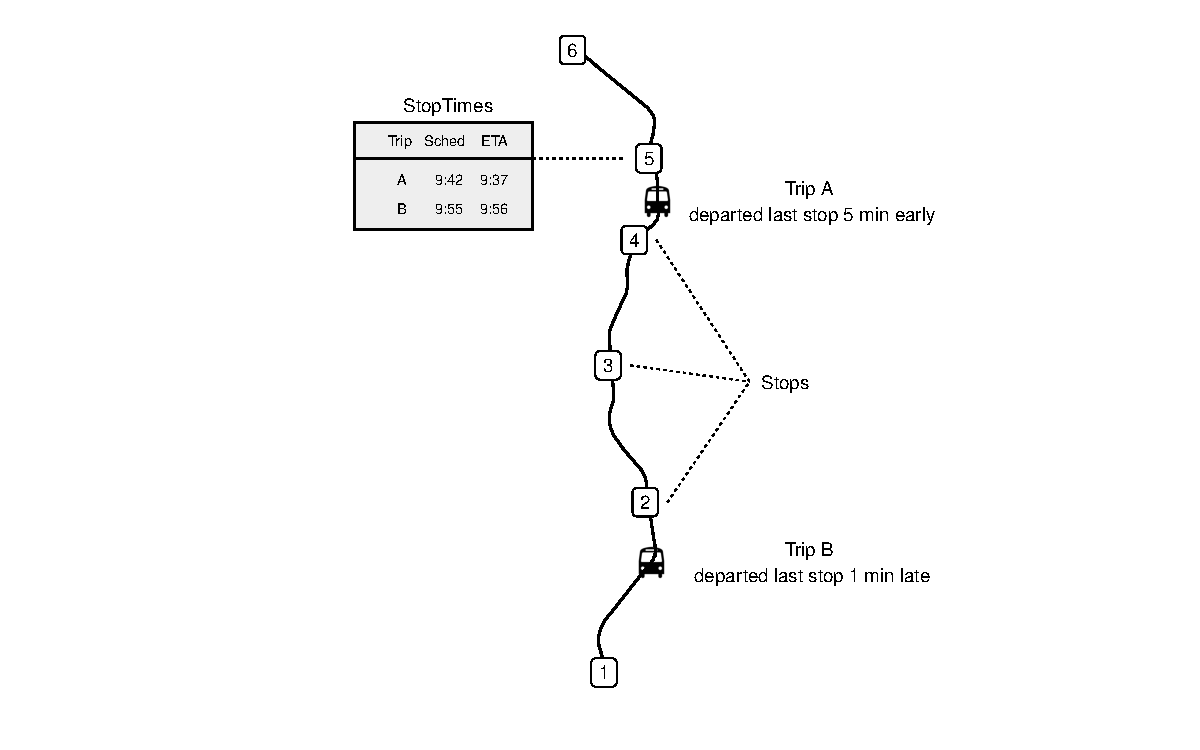
\includegraphics[width=\textwidth]{figure/gtfs_nw-1} 

}

\caption[The main components of a GTFS feed]{The main components of a GTFS feed for a single \emph{route} with two \emph{trips} (A and B) travelling along a \emph{shape} path. The numbered squares represent \emph{stops}, and the scheduled arrival times of each trip at stop 5 are displayed in the \emph{stop times} box.}\label{fig:gtfs_nw}
\end{figure}


\end{knitrout}



Transport providers typically distribute static \GTFS{} data in plain text files, one for each of the components (such as \verb+routes.csv+ and \verb+trips.csv+). Often these are available to download as a single ZIP archive, so the data is easily loaded into a \emph{relational database}, which is described further in \cref{app:gtfs}. The \Rstats{} package developed as part of this work provides the \verb+create_gtfs()+ function to do this automatically:
\begin{knitrout}\small
\definecolor{shadecolor}{rgb}{1, 1, 1}\color{fgcolor}\begin{kframe}
\begin{alltt}
\hlkwd{library}\hlstd{(transitr)}
\hlstd{nw} \hlkwb{<-} \hlkwd{create_gtfs}\hlstd{(}\hlstr{"at_gtfs.zip"}\hlstd{,} \hlkwc{db} \hlstd{=} \hlstr{"at_gtfs.sqlite"}\hlstd{)}
\end{alltt}
\end{kframe}
\end{knitrout}


Within these separate files or tables, the data is stored as per \GTFS{}. Importantly, shapes are stored as sequences of coordinates that draw a path on a map, while stops are represented as a single coordinate marking the location of the bus stop. Stop times are stored in trip-stop pairs with one row for every stop of each trip, along with the scheduled arrival and departure times.\footnote{There are 732,184 rows in the stop times table for Auckland Transport!}



On its own, the static \GTFS{} information can be used like a printed timetable, allowing simple journey planning to take place. As such, it provides a ``fallback'' state in situations where no \rt{} information is available for a given trip: scheduled stop times can be thought of as \emph{prior information}, a core component of the Bayesian paradigm.



\subsection{Real-time GTFS}
\label{sec:gtfs_rt}

The real-time component of \GTFS{} is responsible for handling vehicle positions, trip updates (arrivals at and departures from stops), and service alerts (cancellations and stop closures, for example). Data is processed by a central server and then stored appropriately to enable quick access via \glspl{api}. There is, therefore, the additional need of a server that can handle vast numbers of \gls{api} requests. As such, only a subset of transport providers using \GTFS{} have also implemented the real-time component. Below we give a summary of these components, but further information is available on the \GTFS{} website.\footnote{See \url{https://developers.google.com/transit/gtfs-realtime/}.}


\subsubsection{Vehicle positions}
\label{sec:gtfs_rt_vehicle}

There are several key components to a vehicle position (in the context of \GTFS{}). The \emph{vehicle descriptor} includes information about the physical vehicle, while a \emph{trip descriptor} holds information about the trip being serviced. A \emph{timestamp} specifies exactly when the observation was made, and a \emph{position} contains the actual data, such as the \gls{gps} observation, as is demonstrated by the bus images in \cref{fig:gtfs_nw}.


The specification also allows for additional measurements, such as \emph{speed} or an \emph{odometer} reading. However, these were not available from \AT{} at the time this work was carried out, so they are not included in our application. It is well worth noting, however, that they could be integrated with minimal effort if they become available.


\subsubsection{Trip updates}
\label{sec:gtfs_rt_trip}

As vehicles equipped with \gls{avl} technology arrive at and depart from stops, information about their time of arrival and, most importantly, \emph{schedule adherence} is stored in trip updates. These also contain a \emph{trip descriptor}, as well as one or more \emph{stop time updates}. GTFS-realtime allows storing of stop time updates for all previously visited stops, as well as predictions for upcoming stops. However, Auckland Transport only stores the most recent update.


Each stop time update reports either the arrival or departure time and, where schedule information is available, the schedule adherence by way of an \emph{arrival} or \emph{departure delay} (in seconds). \Cref{fig:gtfs_nw} displays this information offset to the right of each bus location. The on-board \gls{avl} device is responsible for detecting these events, and they are not necessarily linked to the \gls{gps} position of the vehicle. In Auckland, each trip update also triggers a vehicle location update, but the coordinates are those of the \emph{stop}, not of the vehicle. This leads to some of the problems addressed in \cref{sec:realtime-data}.


In Auckland, the current delay is added to the scheduled arrival time, as shown on the \gls{dms} in \cref{fig:gtfs_nw}. We will certainly be discussing the issues associated with this method shortly, and indeed be making comparisons to it throughout the thesis.



\subsubsection{Service alerts}
\label{sec:gtfs_rt_alerts}

Less important for the current work, but essential for reliable \gls{rti}, \emph{service alerts} enable transit operators to modify the static \GTFS{} in real-time. So, when a trip is cancelled, they can send out a service alert announcing the cancellation,\footnote{Although they often don't.} which is then displayed to passengers as a ``C'' on the real-time board. It is also possible to add trips, for example during special events, or to reroute trips around stop closures, but this is beyond the scope of our work.



\subsection{Accessing \rt{} data (API)}
\label{sec:gtfs_rt_api}

Distributing vehicle locations, trip updates, and service alerts to passengers quickly and usefully requires more than just a \gls{dms} at bus stops. Personal mobile devices have revolutionised the way we live our lives, and developers are continually creating new applications to assist with everyday activities. Included in these are transit applications, which are capable of conveying real-time \GTFS{} data to passengers.


The most common method of distributing real-time data is via an \gls{api}. This is, in simple terms, a fixed web address from which developers can request a data file---either \prog{JSON} or, in the case of some \GTFS{} systems, \prog{protobuf}\footnote{See \url{https://developers.google.com/protocol-buffers}}---which can then be parsed and displayed to users. Usually, developers need to register for an \emph{\gls{api} key} which helps to control server demand by limiting the number of requests a user can make, or controlled access to specific data. The \pkg{transitr} package includes the ability to connect to a \GTFS{}-based \gls{api} easily using the following command:
\begin{knitrout}\small
\definecolor{shadecolor}{rgb}{1, 1, 1}\color{fgcolor}\begin{kframe}
\begin{alltt}
\hlstd{url} \hlkwb{<-} \hlstr{"https://api.at.govt.nz/v2/public/realtime/vehiclelocations"}
\hlstd{nw} \hlkwb{<-} \hlkwd{load_gtfs}\hlstd{(}\hlstr{"at_gtfs.sqlite"}\hlstd{)} \hlopt
    \hlkwd{realtime_feed}\hlstd{(url)} \hlopt
    \hlkwd{with_headers}\hlstd{(}
        \hlcom{# this varies by provider}
        \hlstr{"Ocp-Apim-Subscription-Key"} \hlstd{=} \hlkwd{Sys.getenv}\hlstd{(}\hlstr{'APIKEY'}\hlstd{)}
    \hlstd{)}
\end{alltt}
\end{kframe}
\end{knitrout}
